% !TEX root = DesignDocument.tex


\chapter{Project Overview}
This section provides information about the team members, team member roles, project management approach and phase overview.

\section{Team Member's Roles}
Hannah Aker fulfils all team roles, including scrum master, development and testing roles.

\section{Project  Management Approach}
The project will be managed using an Agile approach.  There will be 6 sprints total in this project, each lasting 3 weeks. The project backlog is owned by the team, and located on the team Github repository. All parties have access to the Sprint and Product Backlogs. Github issues will be used to track sprint tasks, bugs or trouble tickets, and user stories. The github repository is located at: \url{https://github.com/SDSMT-CSC464-F15/crowdscience} 


\section{ Stakeholder Information}
Stakeholders for this project are academics and researchers who would use the collected data for research and start new data collections, and ordinary citizens who would be the main users, in the field reporting events. 


\subsection{Customer or End User (Product Owner)}
Product owners are Dr. Mengyu Qiao and Gail Schmidt, who will assist in the project in mentor roles. As needed, they will assist with prioritizing the product backlog, and identify important features. Dr. Mengyu Qiao's research interest area is closely related to crowd-sourcing, and Gail Schmidt was a mentor and sponsor for the original project, the Landscape Change Mapper.

\subsection{Investors}
There are no investors in the project.

\section{Budget}
There is no budget for this project, no new equipment, software, or licence need to be purchased for the completion of this project. Server access is provided by Gail Schmidt.

\section{Intellectual Property and Licensing}
Intellectual property rights belongs to South Dakota School of Mines and Technology. This project is a proof-of-concept project, and will not need special licensing.

\section{Terminology and Acronyms}
\begin{itemize}
\itemsep0em
\item SGT: Stinger Ghaffarian Technologies
\item LCM: Landscape Change Mapper
\item HTML: Hyper-Text Mark-up Language
\item CSS: Cascading Style Sheet
\item PHP: Hypertext Preprocessor
\end{itemize}

\section{Phase  Overview}
This project will be implemented in two phases. The first phase will entail analysing the Landscape Change Mapper project and adapting a copy of the project for expansion into the generic Crowd Science Mapper. The  second phase will entail adding the necessary features to the base project from phase one to create a proof of concept website.

Within phase one, we will implement and then test the adapted Landscape Change Mapper features we add to the project. Delivery is incorporated into the testing phase, because all testing will be done on the live server. Phase two will consist of all the steps in phase one, but will also include a design phase where we fully design the new features to be added.

\section{Sprint Schedule}
There will be 6 sprints, each lasting 3 weeks. The start and end dates for each sprint are listed below.
\begin{itemize}
\itemsep0em
\item Sprint 1: 9/14/15 - 10/2/15
\item Sprint 2: 10/12/15 - 10/30/15
\item Sprint 3: 11/9/15 - 11/27/15
\item Sprint 4: 1/18/15 - 2/5/16
\item Sprint 5: 2/15/16 - 3/4/16
\item Sprint 6: 3/21/16 - 4/15/16
\end{itemize}

\section{Timeline}
See Figure~\ref{projectgantt}.

\begin{figure}[tbh]
\begin{center}
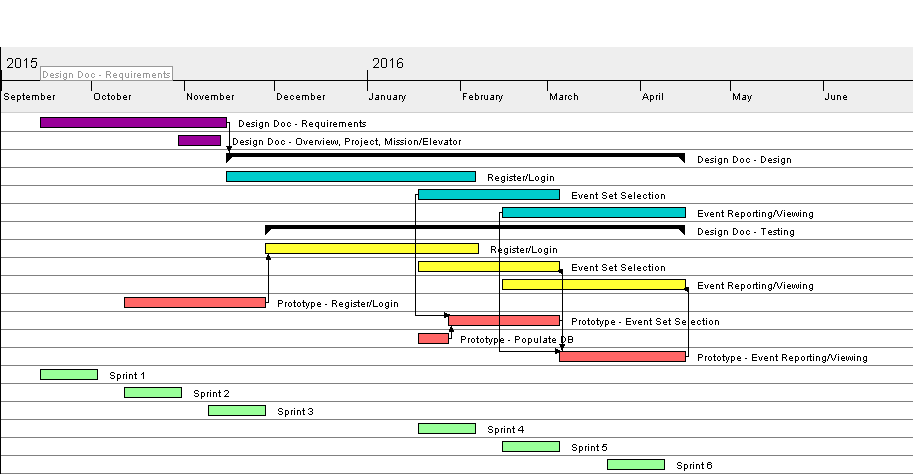
\includegraphics[width=0.75\textwidth]{./figures/projectgantt.png}
\end{center}
\caption{Gantt Chart of Project Completion Schedule\label{projectgantt}}
\end{figure}

\section{Backlogs}

\subsection{Sprint 1 Backlog}
\begin{itemize}
\itemsep0em
\item Documentation: start requirements section.
\item Review code from Landscape Change Mapper project.
\end{itemize}

\subsection{Sprint 2 Backlog}
\begin{itemize}
\itemsep0em
\item Documentation: requirements section, start project, overview and mission/elevator sections.
\item Implement Login/Register interface.
\item Prepare for first client presentation
\end{itemize}

\subsection{Sprint 3 Backlog}
\begin{itemize}
\itemsep0em
\item Documentation: project, overview and mission/elevator sections, start design and testing section for login/register.
\item Finish and test Login/Register interface.
\item Polish design document for first semester review.
\end{itemize}

\subsection{Sprint 4 Backlog}
\begin{itemize}
\itemsep0em
\item Documentation: prototype sections, revise requirements, design and testing section for login/register, start design section for set selection/list, and revised sprint plan in overview.
\item Add sample event reports and sample event set data to database. There will be a collection for each event set, one for information about the event set, and one for user login information.
\item Implement a select box to choose a different event set, and verify that the connection to the database is working as expected. The event report list will be started to verify accuracy of database.
\end{itemize}

\subsection{Sprint 5 Backlog}
\begin{itemize}
\itemsep0em
\item Documentation: design and testing section for set selection/list, start design section for report and map.
\item Implement reporting interface.
\item Finish implementing event report list.
\item Implement map interface.
\end{itemize}

\subsection{Sprint 6 Backlog}
\begin{itemize}
\itemsep0em
\item Finish Documentation: design and testing for report and map features, finalize sprint prototype and sprint report sections.
\item Final testing and debugging.
\item Polish prototype.
\item Design Fair preparation.
\end{itemize}


\section{Development Environment}
This section has information required to set-up a development environment to run, test, and/or develop. 

\subsection{Development IDE and Tools}
No development IDEs were used. Code editing was done in a plain-text editor, Notepad++. More information about Notepad++ can be found at \url{https://notepad-plus-plus.org/}.

\subsection{Source  Control}
Source control is Github; github issues will be used to keep track of backlog and sprint status. The github repository is located at: \url{https://github.com/SDSMT-CSC464-F15/crowdscience} All parties have access to the Sprint and Product Backlogs.

\subsection{Dependencies}
The server requires Apache 2.2 and Mongo DB version 2.4.9 installed to run the project.

\subsection{Build  Environment}
The code in this project does not need to be built. The project uses scripted languages, which do not need compilation or building. 

\subsection{Development Machine Set-up}
A remote desktop connection is required to connect to the server hosting the code. The rdp file for this remote desktop connection is shown in Figure~\ref{alg_rdp}. The development machine should also install a plain-text editor such as Notepad++ to view and edit project files. 
\begin{figure} [tbh]                     
\caption{Remote Desktop Connection (.rdp) file}
\label{alg_rdp}    
\begin{lstlisting}
auto connect:i:1
full address:s: <IP address omitted>
username:s: <username omitted>
password:s: <password omitted>
\end{lstlisting}
\end{figure}


